\documentclass[hidelinks]{article}
\usepackage{stex}

\libinput{preambleCS}

\title{B-Trees}
\author{}
\date{}

\begin{document}

\maketitle

\begin{smodule}[title={B-Trees}]{BTrees}

\symdecl*{B-tree}

\section{Overview}

This note covers the structure and properties of \sns{B-tree}, the basic operations of search, insertion, and deletion, and the main applications of the data structure.

\subsection{Introduction}

\begin{sdefinition}[for=B-tree]
    A \definame{B-tree} is a self-balancing search-tree data structure that maintains sorted data and supports efficient searching, insertion, and deletion. Unlike a binary search tree, every node of a B-tree may store many keys and child pointers, leading to a shallow, balanced tree well-suited to disk-based storage.
\end{sdefinition}

B-trees are the data structure underlying many production database systems (MySQL, PostgreSQL, SQLite) and on-disk file systems (NTFS, macOS HFS+). The ``B'' stands variously for \emph{balanced}, \emph{binary}, or \emph{Bayer}, after the inventors Rudolf Bayer and Edward M.~McCreight.

\subsection{Structure of a B-Tree}

Each node in a \sn{B-tree} can hold many keys and child pointers; for that reason \sns{B-tree} are sometimes called ``large key trees''.
\begin{itemize}
  \item Keys within a node are stored in sorted order, supporting efficient in-node search.
  \item All leaf nodes lie at the same level; the tree is height-balanced.
  \item The number of keys per node is bounded above and below by the order of the tree, which both controls the branching factor and guarantees the time complexity of operations.
\end{itemize}
The combination of a large branching factor and a guaranteed-shallow height means that searches and updates traverse very few nodes from root to leaf even when the data set is enormous.

\subsection{Time Complexity}

The three basic operations all run in time logarithmic in the number of keys $n$:
\[
\begin{array}{l|l}
\text{Operation} & \text{Time complexity}\\
\hline
\text{Search} & O(\log n)\\
\text{Insert} & O(\log n)\\
\text{Delete} & O(\log n)
\end{array}
\]
Search descends the tree from the root, choosing the appropriate child pointer at each level by comparing against the keys stored in the node. Insertion locates the correct leaf and inserts the key there in sorted order, splitting nodes upward when they overflow. Deletion locates the key, removes it, and re-balances the tree by borrowing from a sibling or merging with one when a node would otherwise become underfull.

\subsection{Why Not Just Use a Binary Search Tree?}

A standard \emph{binary search tree} (BST) keeps two child pointers per node and a single key. For data that lives in main memory this is fine, but the assumptions break down at storage scale.

\begin{itemize}
  \item Databases and file systems typically hold data measured in terabytes, while RAM offers only gigabytes; the bulk of the data lives on disk.
  \item Disk reads are roughly five orders of magnitude slower than RAM reads. Concretely, RAM access is on the order of $100\,\text{ns}$, an SSD seek about $100\,\mu s$, and an HDD seek about $10\,\text{ms}$.
\end{itemize}

The \sn{B-tree} solution is to make each node large enough to match a disk page and pack many keys into it. The branching factor $t$ is then in the hundreds or thousands, so the tree height drops to $O(\log_t n)$ and a single root-to-leaf path issues only a handful of disk reads.

\paragraph{Comparison with other balanced structures.}
For $n$ stored keys:
\[
\begin{array}{l|lll}
\text{Structure} & \text{Search} & \text{Insert} & \text{Delete}\\
\hline
\text{Unbalanced BST} & O(n) & O(n) & O(n)\\
\text{AVL tree} & O(\log_2 n) & O(\log_2 n) & O(\log_2 n)\\
\text{Hash table} & O(1) & O(1) & O(1)\\
\text{B-tree} & O(\log_t n) & O(\log_t n) & O(\log_t n)
\end{array}
\]
The hash table wins on asymptotics for unordered lookups but loses ordered traversal, range queries, and locality of disk access. The \sn{B-tree} preserves all three at the cost of a slightly larger constant.

\subsection{Properties of B-Trees}

\begin{itemize}
  \item \textbf{Balanced structure.} A \sn{B-tree} maintains balance by redistributing keys between nodes as necessary, keeping operations efficient.
  \item \textbf{Efficient searching.} Searching is logarithmic in the number of keys thanks to the balance and the in-node sorted order.
  \item \textbf{Efficient insertion and deletion.} The structure adjusts dynamically while maintaining balance, again at logarithmic cost.
  \item \textbf{Optimal disk I/O.} Because each node matches a disk page, the tree minimises the number of pages read or written for any given operation.
\end{itemize}

\subsection{Shape Properties}

A \sn{B-tree} of order $m$ is defined by the following shape properties:
\begin{itemize}
  \item Every node has at most $m$ children.
  \item Every non-leaf node, except possibly the root, has at least $\lceil m/2 \rceil$ children.
  \item The root, if it is not a leaf, has at least two children.
  \item A non-leaf node with $k$ children contains exactly $k-1$ search keys.
  \item Each internal node, except for the root, has between $\lceil m/2 \rceil$ and $m$ children.
  \item All leaves are at the same level, so the tree is height-balanced; leaves carry the actual records (or null pointers, in implementations using external nodes).
\end{itemize}
The lower bound $\lceil m/2 \rceil$ on children for internal nodes is what guarantees the logarithmic time complexity.

\subsection{Worked Example: Order-5 B-Tree}

\begin{example}[An order-5 B-tree]
At order $m = 5$, every internal node carries between $\lceil 5/2 \rceil = 3$ and $5$ children, holding $2$ to $4$ keys. The following tree is a legal order-5 \sn{B-tree}:
\begin{center}
\begin{tikzpicture}[every node/.style={draw, rectangle, minimum height=8mm, inner sep=2mm, font=\small}]
  \node (root) {12};
  \node (l) [below left=1.4cm and 1.5cm of root] {2, 3, 8};
  \node (r) [below right=1.4cm and 1.5cm of root] {13, 27};
  \draw[->] (root) -- (l);
  \draw[->] (root) -- (r);
\end{tikzpicture}
\end{center}
The root holds one key, $12$, and has two children. The left child stores $\{2, 3, 8\}$ and the right child stores $\{13, 27\}$. All leaves sit at the same level, satisfying height balance. The internal-node lower bound is relaxed for the root, which is allowed to have only two children.
\end{example}

\subsection{Insertion}

Insertion proceeds by descending from the root, following the appropriate child at each level just as for search, until a leaf is reached. The new key is placed in that leaf in sorted order. If the leaf has spare capacity the operation is complete; otherwise the leaf is too full and must be split.

\begin{example}[Inserting $10$]
Starting from the order-5 tree above, insert $10$. Searching for $10$ from the root takes the left child of $12$ (since $10 < 12$); within $\{2,3,8\}$ the search ``falls out'' to the right of $8$. The leaf has room ($3$ keys, capacity $4$), so $10$ is added in place:
\begin{center}
\begin{tikzpicture}[every node/.style={draw, rectangle, minimum height=8mm, inner sep=2mm, font=\small}]
  \node (root) {12};
  \node (l) [below left=1.4cm and 1.5cm of root] {2, 3, 8, 10};
  \node (r) [below right=1.4cm and 1.5cm of root] {13, 27};
  \draw[->] (root) -- (l);
  \draw[->] (root) -- (r);
\end{tikzpicture}
\end{center}
\end{example}

\begin{example}[Inserting $11$ via node split]
Continue from the previous state and insert $11$. The search again descends to the left child, but that node is now full (4 keys, the maximum for $m=5$). To accommodate the new key, the leaf is split into two halves around its median. The median key is promoted to the parent, and the parent gains a new child pointer:
\begin{center}
\begin{tikzpicture}[every node/.style={draw, rectangle, minimum height=8mm, inner sep=2mm, font=\small}]
  \node (root) {8, 12};
  \node (l) [below=1.4cm of root, xshift=-3.5cm] {2, 3};
  \node (m) [below=1.4cm of root]                {10, 11};
  \node (r) [below=1.4cm of root, xshift=3.5cm]  {13, 27};
  \draw[->] (root) -- (l);
  \draw[->] (root) -- (m);
  \draw[->] (root) -- (r);
\end{tikzpicture}
\end{center}
The $m+1$ children resulting from the split are divided evenly between the old node and the newly created sibling; the parent gets one new child. If the parent itself overflows, the split propagates upward, possibly all the way to the root (which may itself split, increasing the height of the tree by one).
\end{example}

\subsection{Deletion}

Deletion mirrors insertion: locate the key, remove it, and rebalance if removing it would push a node below its minimum occupancy. Three rebalancing patterns are sufficient for all cases: \emph{borrow from a sibling}, \emph{merge with a sibling}, and (for keys in non-leaf nodes) \emph{replace by predecessor or successor} before deleting from the leaf.

\begin{example}[Deleting $8$ via merge]
Starting from the post-insertion tree above, delete $8$ (which lives in the root). The deletion would normally promote a key from one of the children to take $8$'s place, but neither the left child $\{2,3\}$ nor the middle child $\{10,11\}$ has more keys than the minimum. Instead the two children are merged with the remaining root key $12$ on either side; the result is:
\begin{center}
\begin{tikzpicture}[every node/.style={draw, rectangle, minimum height=8mm, inner sep=2mm, font=\small}]
  \node (root) {12};
  \node (l) [below left=1.4cm and 1.5cm of root]  {2, 3, 10, 11};
  \node (r) [below right=1.4cm and 1.5cm of root] {13, 27};
  \draw[->] (root) -- (l);
  \draw[->] (root) -- (r);
\end{tikzpicture}
\end{center}
\end{example}

\begin{example}[Deleting $13$ by borrowing from a sibling]
Now delete $13$. Removing $13$ would leave the right child with only $\{27\}$, below the minimum-occupancy threshold of two keys. Instead, the deletion borrows: the parent's key $12$ moves down into the right child to replace $13$, and the largest key of the left sibling, $11$, moves up into the parent slot.
\begin{center}
\begin{tikzpicture}[every node/.style={draw, rectangle, minimum height=8mm, inner sep=2mm, font=\small}]
  \node (root) {11};
  \node (l) [below left=1.4cm and 1.5cm of root]  {2, 3, 10};
  \node (r) [below right=1.4cm and 1.5cm of root] {12, 27};
  \draw[->] (root) -- (l);
  \draw[->] (root) -- (r);
\end{tikzpicture}
\end{center}
\end{example}

\begin{example}[Deleting $11$ from an internal node]
To delete $11$, which lives in an internal (non-leaf) node, replace it by the immediately preceding leaf key, here the largest key of the left subtree. That key is $10$, which is in a leaf with spares. The internal occurrence of $11$ is overwritten by $10$, and $10$ is removed from the leaf:
\begin{center}
\begin{tikzpicture}[every node/.style={draw, rectangle, minimum height=8mm, inner sep=2mm, font=\small}]
  \node (root) {10};
  \node (l) [below left=1.4cm and 1.5cm of root]  {2, 3};
  \node (r) [below right=1.4cm and 1.5cm of root] {12, 27};
  \draw[->] (root) -- (l);
  \draw[->] (root) -- (r);
\end{tikzpicture}
\end{center}
\end{example}

\begin{example}[Deleting $2$ via merge and root removal]
Finally delete $2$. Although $2$ lives at leaf level, removing it would underfill the leaf $\{2,3\}$. The leaf has no left sibling and the right sibling $\{12,27\}$ is already at minimum occupancy, so we cannot borrow; instead the two siblings (and their separating key from the root) are merged. The merged leaf now has all five keys, and the root has been emptied of its only key, leaving a stand-alone child:
\begin{center}
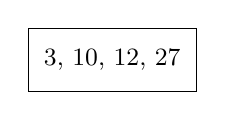
\begin{tikzpicture}[every node/.style={draw, rectangle, minimum height=8mm, inner sep=2mm, font=\small}]
  \node (n) {3, 10, 12, 27};
\end{tikzpicture}
\end{center}
The root no longer satisfies the ``at least two children'' shape constraint, so it is removed and the merged child becomes the new root, reducing the tree's height by one. This is the only way a \sn{B-tree} ever shrinks in height.
\end{example}

\subsection{Applications}

\sns{B-tree} are widely used wherever fast access to large amounts of (often disk-resident) ordered data is required.
\begin{itemize}
  \item Indexing in relational databases and file-system metadata, where the tree's branching factor matches the disk page size.
  \item In-memory and on-disk caches that need ordered traversal in addition to point lookups.
  \item CAD systems use \sns{B-tree} to organise and search geometric data sets that are too large to fit in main memory.
  \item Specialised applications in natural language processing, computer networks, and cryptography rely on \sns{B-tree} when sorted, range-queryable data is required.
\end{itemize}

\subsection{Summary}

A \sn{B-tree} is a self-balancing search tree designed for storage where reads are slow but bulk-block-sized. Search, insert, and delete all run in $O(\log_t n)$ time at the cost of preserving the order-$m$ shape constraints that keep the tree height-balanced. The three basic rebalancing patterns -- splitting on overflow, borrowing from a sibling on underflow, and merging when no sibling has spares -- suffice to maintain those invariants under any sequence of insertions and deletions.

\end{smodule}

\end{document}
